\section{libsnap}

\subsection{libsnap}
\begin{frame}

\only<1>{
  {\Huge \texttt{libsnap}}
}

\only<2->{
\begin{itemize}
  \item<2->freie Implementierung
  \begin{itemize}
    \item<2->GNU Lesser General Public License \textit{(LGPL)}
  \end{itemize}
  \item<3->Hardware- und Plattformunabhängig
  \begin{itemize}
    \item<3->geschrieben in C \textit{(C99, ISO/IEC 9899:1999)}
    \item<3->Buildsystem basiert auf CMake
  \end{itemize}
  \item<4->kleine Codebasis \textit{($\approx$ 3600 LOC)}
  \item<5->einheitliche, saubere API
  \item<6->keine dynamische Speicherallokierung
  \item<7->testgetriebenen Entwicklung
  \begin{itemize}
    \item<7->basiert auf dem CUnit Testing Framework
    \item<7->CTest - integriert im Build-Prozess
    \item<7->60\% Code sind Tests \textit{($\approx$ 2200 LOC)}
    \item<7->gcov/lcov basierter Coverage Report
    \item<7->dadurch $\approx$ 100\% Testabdeckung
  \end{itemize}
\end{itemize}
}
\end{frame}


\subsection{coverage}
\begin{frame}[fragile]
\begin{center}
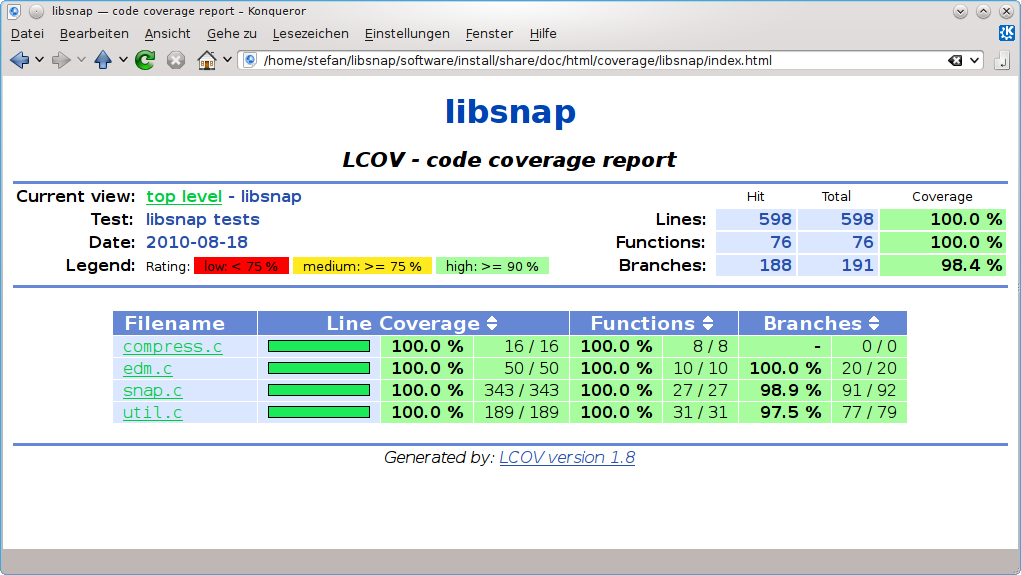
\includegraphics[scale=0.4]{images/lcov_1.png}
\end{center}
\end{frame}

\subsection{snap\_encode}
\begin{frame}[fragile]
\lstinputlisting[]{sources/encode.h}
\end{frame}


\subsection{snap\_encode\_bound}
\begin{frame}[fragile]
\lstinputlisting[]{sources/encode_bound.h}
\end{frame}


\subsection{snap\_decode}
\begin{frame}[fragile]
\lstinputlisting[]{sources/decode.h}
\end{frame}


\subsection{snap\_decode\_bound}
\begin{frame}[fragile]
\lstinputlisting[]{sources/decode_bound.h}
\end{frame}


\subsection{snap_example}
\begin{frame}[fragile]
\lstinputlisting[basicstyle =\ttfamily\footnotesize\mdseries]{sources/snap_example.c}
\end{frame}


\subsection{snap\_\ast}
\begin{frame}[fragile]
\lstinputlisting[basicstyle =\ttfamily\scriptsize\mdseries]{sources/snap_functions.h}
\end{frame}

\subsection{Issues}
\begin{frame}[fragile]
  \begin{itemize}
    \item<1->Das \texttt{EDM}-Flag kann unbemerkt kippen
    \item<2->Vorw\"artsfehlerkorrektur \texttt{FEC} wird erw\"ahnt, aber nicht spezifiziert
    \item<3->ein C-String wird ohne \texttt{NULL}-Terminierung dekodiert!
    \item<4->\texttt{encode} kann \"uber 100\% Overhead erzeugen
  \end{itemize}
\end{frame}
% kate: word-wrap off; encoding utf-8; indent-width 4; tab-width 4; line-numbers on; mixed-indent off; remove-trailing-space-save on; replace-tabs-save on; replace-tabs on; space-indent on;
% vim:set spell et sw=4 ts=4 nowrap cino=l1,cs,U1:
